\chapter{Realisierung Objekt Erkennung}\label{kap:object_det}

\section{Datensatz}\label{sec:dataset}

Um ein Deep Learning Modell richtig trainieren zu können, 
wird eine große Menge an gelabelten Trainingsdaten benötigt.
Im Falle der Objekterkennung enthalten die labels neben der 
Klasse auch die Koordinaten der Bounding Boxen, 
welche das zu erkennende Objekt auf dem Bild umrahmen.


Für die vorliegende Arbeit wurden dafür aus dem Open Source 
Dataset \textit{OpenImages} \cite{kuznetsovaOpenImagesDataset2018} 
von Google 9 Klassen, welche Wildtiere enthalten heruntergeladen.

Dieses besteht aus einem Trainingsset mit 200 bis 2000 Bildern pro 
Klasse sowie kleineren Test- und Validierungssets. Um für alle Klassen 
die gleiche Anzahl an Trainingsdaten zu erhalten und um Overfitting zu 
verhindern wurden wie im folgenden beschrieben die Trainingsdaten 
augmentiert.

\subsection{Augmentierung}

Augmentierung ist eine Technik, mit der aus den vorhandenen 
Daten künstlich mehr Daten generiert werden können. Dafür werden 
z.B. geometrische Transormationen, wie etwa Sklierung, Verschiebung 
Rotieren und Spiegelungen oder manipulationen der Pixelwerte 
zur veränderung der Farbwerte, Helligkeit, Kontrast oder 
Rauschen vorgenommen.

Mithilfe eines Python Scripts und der Library \textit{imgaug} \cite{imgaug}
konnten so verschiedene Augmentierungstechniken auf das Datenset angewendet
werden.

\begin{figure}[H]
    \centering
    \label{fig:augmentierung}
    \includegraphics[width=0.8\columnwidth]{Bilder/augmentierung.png}
    \caption{Anwendung von Augmentierungstechniken}
\end{figure}


\section{Training}

Da der Neural Compute Stick mit OpenVino ein eigenes Datei Format 
für die traininerten Modelle verwendet, musste bei der Auswahl
eines Frameworks sowie Models auf die Kompatibilität zu OpenVino 
geachtet werden. 

% Verwendete wurde daher das untersstütze Framework Tensorflow, 
% um zwei Ansätze zu verfolgen. Der eine verwendet die Api Keras, 
% und versucht neben der Klassifikation die Lokalisierung mit 
% dieser vorzunahemen, der andere verwendet eine speziell für die 
% Objekterkennung konzipierte Api für wie in Abschnitt
%  \ref{sec:related_work} beschriebene End-to-End lösungen.


\subsection{Tensorflow Object Detection Api}

Die Tensorflow Object Detection Api ist unter den Research Modellen
\cite{tfobjdet} des offiziellen Tensorflow Repository zu
finden und enthällt implementierungen einiger gängiger Object Detectin
Modelle, wie Single Shot Detectors (SSD) und Faster R-CNNs mit 
verschiedenen Basis CNNs mit vortrainierten Geweichten.

Um die Modelle trainieren zu können, mussten zunächst die 
Trainingsdaten in das binary Dateiformate TFRecords umgewandelt 
werden, welches die Api verwendet. Dieses ist eine Serialisierte 
darstellung der Bilder und Labels als Protocol Buffer für
effizienten Zugriff auf diese.

Trainiert wurde mit hilfe \textit{Google Colab}, eine cloudbasierte VM,
welche eine geeignete Gpu zur verfügung stellt.


\subsection{Trainingsworkflow}

Das Ergebnis des Trainings kann neben der Auswahl eines geeigneten 
Modell, sowie auswahl und aufbereitung des Datensatzes auch durch 
anpassungen sogenannter Hyperparameter beeinflusst werden.

Mit diesen können in \ref{subsec:validation} beschriebene 
Verfahren realisiert werden.

Durch eine Evaluierung zur Laufzeit des Trainings können so Fehler 
in der Konfigureation des Trainings erkannt und durch anpassen von 
entweder Datensatz, Modell oder Parameter korrigiert/verbessert 
werden.
Es ergibt sich folgender Workflow.

% \begin{figure}[H]
%     \centering
%     \def\svgwidth{0.7\textwidth}
%     
\tikzstyle{process} = [rectangle, fill=blue!20, node distance=4cm, minimum width=1.5cm, minimum height=0.8cm, text centered, draw=black]
\tikzstyle{arrow} = [thick,->,>=stealth]
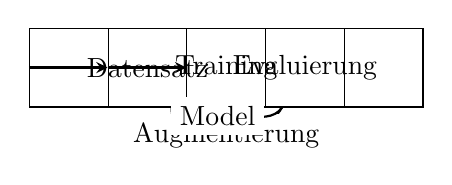
\begin{tikzpicture}[scale=0.4]
      \node (data)      [process]                   {Datensatz};
      \node (train)      [process, right of=data]      {Training};
      \node (eval)      [process, right of=train]      {Evaluierung};
    \draw[arrow] (data) -- (train);
    \draw[arrow] (train) -- (eval);
  \draw[arrow] (eval) edge[bend left=60] node [centered, fill=white!30] {Augmentierung} (data);
  \draw[arrow] (eval) edge[bend left=60] node [left, fill=white!30] {Model} (train);
\end{tikzpicture}

% \begin{tikzpicture}[scale=0.4]

%   \begin{scope}[node distance=3cm]

%    \node (data)      [process]                   {Datensatz};
%    \node (prep)      [process, right of=data]      {Aufbereitung};
%    \node (model)      [process, right of=prep]      {Model};
%    \node (train)      [process, right of=model]      {Training};
%    \node (eval)      [process, right of=train]      {Evaluierung};

%   \end{scope}

%  \draw[arrow] (data) -- (prep);
%  \draw[arrow] (prep) -- (model);
%  \draw[arrow] (model) -- (train);
%  \draw[arrow] (train) -- (eval);
 

% \draw[arrow] (eval) edge[bend left=60] node [left, fill=white!30] {ändern} (data);
% \draw[arrow] (eval) edge[bend left=60] node [left, fill=white!30] {augment} (prep);
% \draw[arrow] (eval) edge[bend left=60] node [left, fill=white!30] {ändern} (model);
% \draw[arrow] (eval) edge[bend left=60] node [left, fill=white!30] {Parameter} (train);

 
% \end{tikzpicture}

%     \caption{Trainingsworkflow}
%     \label{fig:train_workflow}
% \end{figure}

% \vspace{1cm}

\begin{figure}[H]
    \centering
    
\tikzstyle{process} = [rectangle, fill=blue!20, node distance=4cm, minimum width=1.5cm, minimum height=0.8cm, text centered, draw=black]
\tikzstyle{arrow} = [thick,->,>=stealth]
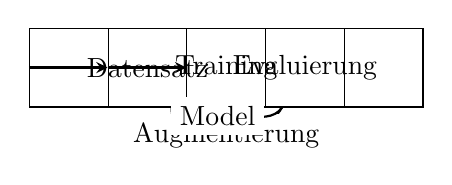
\begin{tikzpicture}[scale=0.4]
      \node (data)      [process]                   {Datensatz};
      \node (train)      [process, right of=data]      {Training};
      \node (eval)      [process, right of=train]      {Evaluierung};
    \draw[arrow] (data) -- (train);
    \draw[arrow] (train) -- (eval);
  \draw[arrow] (eval) edge[bend left=60] node [centered, fill=white!30] {Augmentierung} (data);
  \draw[arrow] (eval) edge[bend left=60] node [left, fill=white!30] {Model} (train);
\end{tikzpicture}

% \begin{tikzpicture}[scale=0.4]

%   \begin{scope}[node distance=3cm]

%    \node (data)      [process]                   {Datensatz};
%    \node (prep)      [process, right of=data]      {Aufbereitung};
%    \node (model)      [process, right of=prep]      {Model};
%    \node (train)      [process, right of=model]      {Training};
%    \node (eval)      [process, right of=train]      {Evaluierung};

%   \end{scope}

%  \draw[arrow] (data) -- (prep);
%  \draw[arrow] (prep) -- (model);
%  \draw[arrow] (model) -- (train);
%  \draw[arrow] (train) -- (eval);
 

% \draw[arrow] (eval) edge[bend left=60] node [left, fill=white!30] {ändern} (data);
% \draw[arrow] (eval) edge[bend left=60] node [left, fill=white!30] {augment} (prep);
% \draw[arrow] (eval) edge[bend left=60] node [left, fill=white!30] {ändern} (model);
% \draw[arrow] (eval) edge[bend left=60] node [left, fill=white!30] {Parameter} (train);

 
% \end{tikzpicture}

    \caption{Trainingsworkflow}
    \label{fig:train_workflow}
\end{figure}


Die Ergebnisse werden im nächsten Kapitel (\ref{kap:eval}) diskutiert.

\section{Inferenz}

\begin{itemize}
    \item Tensorflow graph exportieren/einfrieren
    \item mit model opt in ir Format
    \item mit inf engine inferieren
\end{itemize}


\subsection{OpenVinos InferecneEgine}

Folgend der prinzipielle Ablauf der Inference Engine für 
die Inferenz eines Modells auf dem Neural Comput Stick


\begin{minipage}{0.30\textwidth}
    \centering
    
\tikzstyle{process} = [rectangle, minimum width=3cm, minimum height=1cm, text centered, draw=black]
\tikzstyle{arrow} = [thick,->,>=stealth]

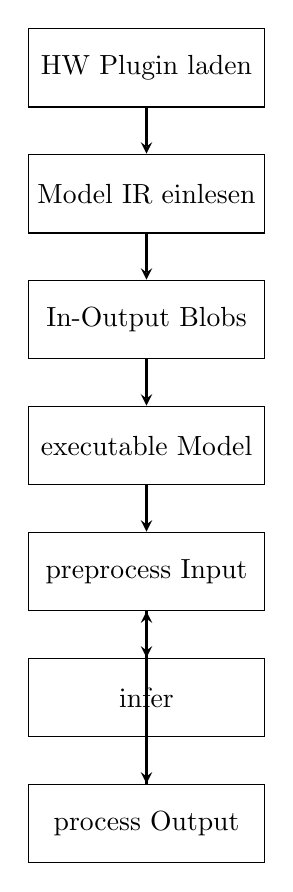
\begin{tikzpicture}[node distance=1.6cm]
    \node (hw)      [process]                   {HW Plugin laden};
    \node (ir)      [process, below of=hw]      {Model IR einlesen};
    \node (io)      [process, below of=ir]      {In-Output Blobs};
    \node (execNet) [process, below of=io]      {executable Model};
    \node (prepIn)  [process, below of=execNet] {preprocess Input};
    \node (infer)   [process, below of=prepIn]  {infer};
    \node (procOut) [process, below of=infer]   {process Output};

    \draw [arrow] (hw) -- (ir);
    \draw [arrow] (ir) -- (io);
    \draw [arrow] (io) -- (execNet);
    \draw [arrow] (execNet) -- (prepIn);
    \draw [arrow] (prepIn) -- (infer);
    \draw [arrow] (infer) -- (procOut);
    \draw [arrow] (procOut) -- (prepIn);
    
\end{tikzpicture}

    \captionof{figure}{}
    \label{}
\end{minipage}
\begin{minipage}{0.70\textwidth}

%\begin{python}
\begin{lstlisting}[language=Python]

    plugin = IEPlugin(device='MYRIAD')

        
    net = IENetwork(model_xml, model_bin)
        
    
    input_blob  = net.inputs
    output_blob = net.outputs
        

    exec_net = plugin.load_network(net, n_req)
        
    while True:

        image = preprocess(capture) # hwc -> nchw
        
        
        res = exec_net.infer({input_blob : image})
        

        res = res[output_blob] #
        
        
\end{lstlisting}
%\end{python}
\vspace{1.5cm}
\end{minipage}

% transform:
% # capture dims zu input blob dims transformieren
% # img_h, img_w, img_c -> blob_n, blob_c, blob_h, blob_w

Output Format variert je nach Modell, Image Classification,
ObjectDetection sowie Instance Segmentation.


Für Object Detection Modelle 
enthällt eine Liste mit allen möglichen erkannten Objekten, jedes 
davon bestehend aus einem Array mit den Indices:

\begin{enumerate}
    \setcounter{enumi}{-1}
    \item batch index
    \item class label
    \item Wahrscheinlichkeit
    \item $x_{min}$ Box Koordinate
    \item $y_{min}$ Box Koordinate
    \item $x_{max}$ Box Koordinate
    \item $y_{max}$ Box Koordinate
\end{enumerate}


\subsubsection{Asynchrone Inferenz}


Um die Ausführungzeit der Inferenz zu verringern, können, 
je nach Hardware Optimierungen wie Asynchtone Inferenz, 
Inferenz requests auf mehreren Threads, oder Batching des 
Inputs vorgenommen werden.

\begin{figure}[htb]
    \centering
    \def\svgwidth{0.7\textwidth}
    \input{Bilder/synch_asynch.pdf_tex}
    \caption{Asynchron und mehrerere Inferenz Requests}
    \label{fig:async}
\end{figure}

In Abbildung \ref{fig:async} dargestellt die Asynchrone ausführung 
zwischen dem aufbereiten der Frames und der Inferenz, sowie 
mehrere parallel ausgeführte Inferenz Requests.

